\documentclass{article}
\usepackage{graphicx} % Required for inserting images
\usepackage{amsmath}
\usepackage{hyperref}
\usepackage{caption}
\usepackage{subcaption}
\usepackage{circuitikz}

\title{EE1204 Assignment 1}
\author{Arjun Pavanje}
\date{March 2025}

\begin{document}

\maketitle

1. Two point charges of equal magnitude $q$ are positioned at $z = \pm \frac{d}{2}$. We aim to determine:
\begin{enumerate}
    \item[(a)] The electric field everywhere on the $z$-axis.
    \item[(b)] The electric field everywhere on the $x$-axis.
    \item[(c)] The results of (a) and (b) if the charge at $z = -\frac{d}{2}$ is $-1C$ instead of $1C$.
\end{enumerate}

\textbf{Solution:}\newline
\textbf{(a)} 
\begin{figure}[!ht]
\centering
\resizebox{0.5\textwidth}{!}{%
\begin{circuitikz}
\tikzstyle{every node}=[font=\normalsize]
\draw  (8.75,10.5) circle (0.25cm);
\draw  (13.75,10.5) circle (0.25cm);
\draw [<->, >=Stealth] (7.5,10.5) -- (15,10.5);
\draw [<->, >=Stealth] (11.25,7.5) -- (11.25,13.75);
\node [font=\normalsize] at (8.75,9.75) {$Q_1$};
\node [font=\normalsize] at (13.75,9.75) {$Q_2$};
\node [font=\normalsize] at (12.25,11) {$(0, 0, z)$};
\node [font=\normalsize] at (11.25,14) {$x$};
\node [font=\normalsize] at (15.25,10.5) {$z$};
\draw [->, >=Stealth, dashed] (8.75,10.5) -- (12,10.5);
\draw [->, >=Stealth, dashed] (13.75,10.5) -- (12,10.5);
\end{circuitikz}
}%

\label{fig:my_label}
\end{figure}
Field on z-axis ($E$): $E = E_1 + E_2$

\begin{itemize}
    \item $E_1$: Field due to $Q_1$
    \item $E_2$: Field due to $Q_2$
\end{itemize}

\begin{align*}
E_1 &= \frac{q}{4 \pi \epsilon_0} \frac{|x-\frac{d}{2}| }{(x - \frac{d}{2})^3} \hat{k}, \quad
E_2 = -\frac{q}{4 \pi \epsilon_0} \frac{|x + \frac{d}{2}|}{(x + \frac{d}{2})^3} \mathbf{\hat{k}} \\
E &= E_1 + E_2 = \frac{q}{4 \pi \epsilon_0} 
\left[ 
\frac{|x - \frac{d}{2}|}{(x - \frac{d}{2})^3} - \frac{|x + \frac{d}{2}|}{(x + \frac{d}{2})^3}
\right]\mathbf{\hat{k}}
\end{align*}

Case 1: $z > \frac{d}{2}$

\begin{align*}
E &= \frac{q}{2 \pi \epsilon_0} 
\left[ 
\frac{z^2 + (\frac{d}{2})^2}{(z^2 - (\frac{d}{2})^2)^2}
\right] \mathbf{(\hat{k})}
\end{align*}

Case 2: $z < -\frac{d}{2}$

\begin{align*}
E &= \frac{q}{2 \pi \epsilon_0} 
\left[ 
\frac{z^2 + (\frac{d}{2})^2}{(z^2 - (\frac{d}{2})^2)^2}
\right] (-\mathbf{\hat{k}})
\end{align*}

Case 3: $-\frac{d}{2} < z < \frac{d}{2}$

\begin{align*}
E &= \frac{q}{2 \pi \epsilon_0} 
\left[ 
\frac{1}{(z + \frac{d}{2})^2} - \frac{1}{(z - \frac{d}{2})^2}
\right] (\mathbf{\hat{k}})\\
&= \frac{q}{2 \pi \epsilon_0} 
\left[ 
\frac{zd}{(z^2 - (\frac{d}{2})^2)^2}
\right] (-\mathbf{\hat{k}})
\end{align*}

\textbf{(b)}
\begin{figure}[!ht]
\centering
\resizebox{0.5\textwidth}{!}{%
\begin{circuitikz}
\tikzstyle{every node}=[font=\normalsize]
\draw  (8.75,10.5) circle (0.25cm);
\draw  (13.75,10.5) circle (0.25cm);
\draw [<->, >=Stealth] (7.5,10.5) -- (15,10.5);
\draw [<->, >=Stealth] (11.25,7.5) -- (11.25,13.75);
\draw [->, >=Stealth, dashed] (8.75,10.5) -- (12.5,13);
\draw [->, >=Stealth, dashed] (13.75,10.5) -- (10,13);
\node [font=\normalsize] at (8.75,9.75) {$Q_1$};
\node [font=\normalsize] at (13.75,9.75) {$Q_2$};
\node [font=\normalsize] at (12.5,12.25) {$(x, 0, 0)$};
\node [font=\normalsize] at (11.25,14) {$x$};
\node [font=\normalsize] at (15.25,10.5) {$z$};
\end{circuitikz}
}%

\label{fig:my_label}
\end{figure}
\begin{align*}
\text{Field on x-axis (E): } & \, E_1 + E_2 \\
E_1: \text{Field due to } q_1, & \quad E_2: \text{Field due to } q_2 \\
E &= \frac{q}{4 \pi \epsilon_0} 
\left( 
\frac{x\hat{i} - \frac{d}{2} \hat{k}}{\left(x^2 + \left(\frac{d}{2}\right)^2\right)^{3/2}} 
+ 
\frac{\left(x \hat{i} + \frac{d}{2}\hat{k}\right)}{\left(x^2 + \left(\frac{d}{2}\right)^2\right)^{3/2}}
\right) \mathbf{\hat{i}}
\\
E &= \frac{q}{2 \pi \epsilon_0} 
\frac{x}{\left(x^2 + \left(\frac{d}{2}\right)^2\right)^{3/2}} \mathbf{\hat{i}}.
\end{align*}
\textbf{\text{(c)}} Result obtained in $(a)$ becomes,\newline 
Case 1: $z > \frac{d}{2}$,
\begin{align*}
E &= \frac{q}{4 \pi \epsilon_0} 
\left( 
\frac{1}{(z - \frac{d}{2})^2} - 
\frac{1}{(z + \frac{d}{2})^2}
\right) \mathbf{\hat{k}} \\ 
E &= \frac{q}{2 \pi \epsilon_0} 
\frac{zd}{(z^2 - (\frac{d}{2})^2)^2} \mathbf{\hat{k}}.
\end{align*}
Case 2: $z < -\frac{d}{2}$, 
\begin{align*}
E &= +\frac{q}{4 \pi \epsilon_0} 
\left( 
\frac{zd}{(z^2 - (\frac{d}{2})^2)^3} )
\right)-\mathbf{\hat{k}}
\end{align*}
Case 3: $-\frac{d}{2} < z < \frac{d}{2}$
\begin{align*}
E &= -\frac{q}{4 \pi \epsilon_0} 
\left( 
\frac{1}{(z + \frac{d}{2})^2} + 
\frac{1}{(z - \frac{d}{2})^2}
\right) \mathbf{\hat{k}} \\ 
&= -\frac{q}{4 \pi \epsilon_0} 
\left( 
\frac{z^2 + (\frac{d}{2})^2}{ (z^2 - (\frac{d}{2})^2)^2 } \right) \mathbf{\hat{k}}
\end{align*}
Result obtained in $(b)$ becomes,
\begin{align*}
E &= \frac{q}{4 \pi \epsilon_0} 
\left( 
\frac{x\hat{i} - \frac{d}{2} \hat{k}}{\left(x^2 + \left(\frac{d}{2}\right)^2\right)^{3/2}} 
- 
\frac{\left(x \hat{i} + \frac{d}{2}\hat{k}\right)}{\left(x^2 + \left(\frac{d}{2}\right)^2\right)^{3/2}}
\right) \mathbf{\hat{i}} 
\\
E &= \frac{q}{4 \pi \epsilon_0} 
\frac{d}{\left(x^2 + \left(\frac{d}{2}\right)^2\right)^{3/2}} (-\mathbf{\hat{i}}).
\end{align*}

2. A crude device for measuring charge consists of two small insulating spheres of radius $a$, one of which is fixed in position. The other is movable along the $x$-axis and is subject to a restraining force $kx$, where $k$ is a spring constant. The uncharged spheres are centered at $x = 0$ and $x = d$, the latter fixed. If the spheres are given equal and opposite charges of $Q/C$, obtain the expression by which $Q$ may be found as a function of $x$. Determine the maximum charge that can be measured in terms of $\epsilon_0$, $k$, and $d$, and then state the separation of the spheres. What happens if a larger charge is applied? \newline
\textbf{Solution:} \newline
\begin{figure}[!ht]
\centering
\resizebox{0.75\textwidth}{!}{%
\begin{circuitikz}
\tikzstyle{every node}=[font=\normalsize]
\draw  (5,11.75) circle (1.25cm);
\draw  (12.5,11.75) circle (1.25cm);
\node [font=\normalsize] at (5,10) {$x = 0$};
\node [font=\normalsize] at (12.5,10) {$x = d$};
\draw [->, >=Stealth] (5,11.75) -- (7,11.75)node[pos=0.5, fill=white]{$F_{columb}$};
\draw [->, >=Stealth] (5,11.75) -- (3.25,11.75)node[pos=0.5, fill=white]{$F_{spring}$};
\draw [->, >=Stealth, dashed] (7,11.75) -- (15.25,11.75);
\draw [->, >=Stealth, dashed] (3.25,11.75) -- (2.25,11.75);
\end{circuitikz}
}%

\label{fig:my_label}
\end{figure}
Say $Q_1 = +Q$ is the movable charge, $Q_2 = -Q$ is the stationary charge.

At equilibrium, moving force on $Q$ is balanced by electrostatic force:
\begin{align*}
\frac{1}{4 \pi \epsilon_0} \frac{Q^2}{(x-d)^2} = kx
\end{align*}

\begin{align*}
Q = \sqrt{4 \pi \epsilon_0 k x (x-d)^2}
\end{align*}

Maximum measurable charge:
\begin{align*}
\frac{dQ}{dx} = 0
\end{align*}

Differentiating,
\begin{align*}
(x-d)^2 \left( x - \frac{d}{3} \right) = 0
\end{align*}

\begin{align*}
x = d \quad \text{(minimum)}
\end{align*}

\begin{align*}
x = \frac{d}{3} \quad \text{(maximum)}
\end{align*}

\begin{align*}
Q_{\text{max}} = \sqrt{\frac{16\pi \epsilon_0 k d^3}{9}}
\end{align*}

Seperation,
\begin{align*}
x = \frac{2d}{3}
\end{align*}



3. A flux density field is given as
\begin{align*}
\mathbf{F}_1 = 5\mathbf{a_z}.
\end{align*}

The task is to evaluate the outward flux of $\mathbf{F}_1$ through the hemispherical surface defined by $r = a$, $0 < \theta < \pi/2$, and $0 < \phi < 2\pi$. Next, consider what simple observation would have saved a lot of work in the previous part. Identifying symmetries or using alternative methods can simplify the calculations significantly.

Now suppose the field is given by
\begin{align*}
\mathbf{F}_2 = 5z \mathbf{a_z}.
\end{align*}

Using the appropriate surface integrals, determine the net outward flux of $\mathbf{F}_2$ through the closed surface consisting of the hemisphere from the first part and its circular base in the $xy$ plane. Finally, repeat the previous calculation by applying the divergence theorem and evaluating an appropriate volume integral. This approach should confirm the result obtained through direct surface integration.

\textbf{Solution:}\newline
\begin{figure}[h!]
   \centering
   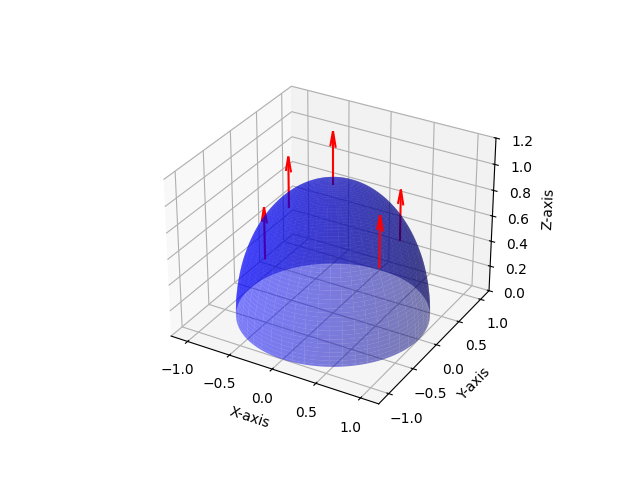
\includegraphics[width=1\columnwidth]{figs/q3.png}
    \caption{Hemisphere, Field lines}
   \label{label}
\end{figure}

Flux due to electric field over a surface $S$:
\begin{align*}
\iint \vec{E} \cdot \vec{n} \, dS
\end{align*}

Here, the surface is a hemispherical surface. Using spherical coordinates:
\begin{align*}
\vec{E} &= 5z \hat{k}, \\
\vec{n} &= \frac{x}{\sqrt{x^2 + y^2 + z^2}} \hat{i} + \frac{y}{\sqrt{x^2 + y^2 + z^2}} \hat{j} + \frac{z}{\sqrt{x^2 + y^2 + z^2}} \hat{k}
\end{align*}
In spherical coordinates,
\begin{align*}
    x &= \rho \sin(\theta)  \cos(\phi)\\
    y &= \rho \sin(\theta)  \sin(\phi)\\
    z &= \rho \cos(\theta)
\end{align*}
Thus,
\begin{align*}
dS &= a^2 \sin{\theta} \, d\theta \, d\phi
\end{align*}

The flux becomes:
\begin{align*}
&= \iint 5a^2 \cos{\theta} \sin{\theta} \, d\theta \, d\phi
\end{align*}

Separating the integrals:
\begin{align*}
&= 5a^2 \int_{0}^{2\pi} d\phi \int_{0}^{\pi/2} \cos{\theta} \sin{\theta} \, d\theta
\end{align*}

For the $\theta$ integral:
\begin{align*}
&= 5a^2 \int_{0}^{2\pi} d\phi \left[ -\frac{\cos^2{\theta}}{2} \right]_{0}^{\pi/2} \\
&= 5a^2 \int_{0}^{2\pi} d\phi \cdot \frac{1}{2} \\
&= 5\pi a^2
\end{align*}
There is an easier way to find flux, we can say that flux passing through the hemisphere is the same as that passing through a disc of radius $a$ centered at
the origin as both surfaces subtend the same solid angle.

\begin{align*}
\text{Flux} &= \iint \vec{E} \cdot \vec{n} \, dS \\
\vec{E} \cdot \vec{n} & = 5 \\
\text{Flux } &= 5 \iint dS \\
& = 5 (\pi a^2)
\end{align*}
This is the same result obtained above by integration. Now if field changes to $E = 5z\hat{k}$,
\begin{align*}
\vec{E} = 5z \hat{k}, \quad \hat{n} = \frac{x \hat{i} + y \hat{j} + z \hat{k}}{\sqrt{x^2 + y^2 + z^2}}
\end{align*}

Flux:
\begin{align*}
\text{Flux} = \iint_S \vec{E} \cdot \hat{n} \, dS
\end{align*}

Substituting:
\begin{align*}
\text{Flux} = \int_0^{2\pi} \int_0^{\pi} 5a^3 \cos^2\theta \, a^2 \sin\theta \, d\theta d\phi
\end{align*}

Simplifying,
\begin{align*}
= \int_0^{2\pi}  \int_0^{\pi/2} 5a^3 \cos^2\theta \sin\theta \, d\theta d\phi
= \int_0^{2\pi}   \left[-\frac{5a^3}{3} cos(\theta)\right]_0^{\pi/2} d\phi
\end{align*}

Using substitution:
\begin{align*}
= 5a^3 \cdot 2\pi \cdot \frac{1}{3}
= \frac{10}{3}\pi a^3
\end{align*}

\vspace{1cm}

Applying Divergence Theorem:

Flux:
\begin{align*}
\text{Flux} = \iint_S (\vec{E} \cdot \hat{n}) dS = \iiint_V (\nabla \cdot \vec{E}) dV
\end{align*}

Calculate divergence:
\begin{align*}
\nabla \cdot \vec{E} = 
    \frac{\partial}{\partial x}(0) +
    \frac{\partial}{\partial y}(0) +
    \frac{\partial}{\partial z}(5z) = 5
\end{align*}

Volume integral:
\begin{align*}
\text{Flux} = 5 \iiint_V dV
= 5 \left[\frac{2}{3}\pi a^3\right]
= 5a^3
= \frac{10}{3} \pi a^3
\end{align*}
This verifies the result obtained by direct integration.
\newline \newline

4. An infinitely long cylindrical dielectric of radius $b$ contains charge within its volume with a charge density given by
\begin{align*}
\rho_v = a \rho^2,
\end{align*}
where $a$ is a constant. The goal is to determine the electric field strength $\mathbf{E}$ both inside and outside the cylinder.\newline
\textbf{Solution: }\newline
\begin{figure}[h!]
   \centering
   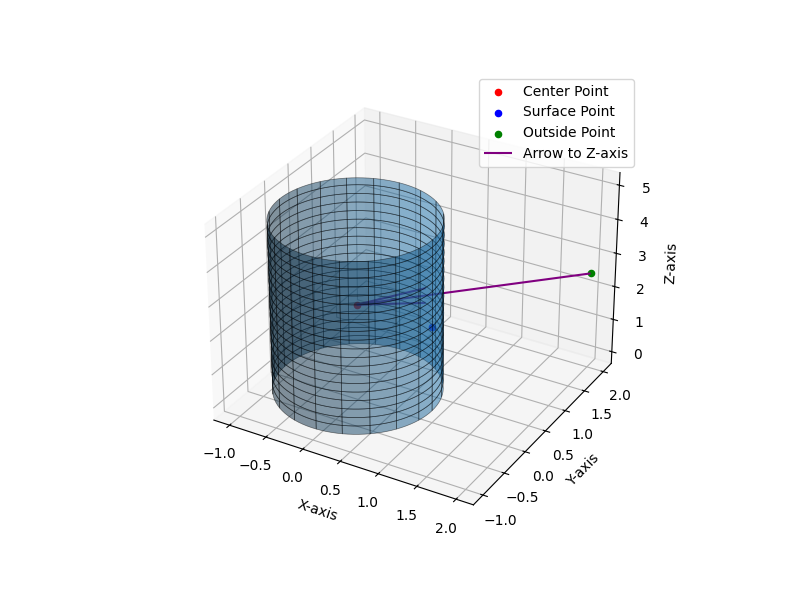
\includegraphics[width=1\columnwidth]{figs/q4.png}
    \caption{Cylinder}
   \label{label}
\end{figure}
We can solve this problem using Gauss's law,
\begin{align*}
\iint \vec{E} \cdot \vec{dS} = \frac{Q_{\text{enc}}}{\epsilon_0}.
\end{align*}

For $ Q_{\text{enc}} $:
\begin{align*}
Q_{\text{enc}} = \int_0^l \int_0^{2\pi} \int_0^r a x^3 r \, dr \, d\phi \, dz,
\end{align*}
where $ x = r $.

Simplifying:
\begin{align*}
Q_{\text{enc}} = \int_{z=0}^l \int_{\phi=0}^{2\pi} \int_{r=0}^r a r^4 \, dr \, d\phi \, dz.
\end{align*}
\begin{align*}
Q_{\text{enc}} = \int_0^l \int_0^{2\pi} \frac{a r^5}{5} \Big|_0^r d\phi dz.
\end{align*}
\begin{align*}
Q_{\text{enc}} = \int_0^l \int_0^{2\pi} \frac{a r^5}{5} d\phi dz.
\end{align*}
\begin{align*}
Q_{\text{enc}} = (2\pi l) \frac{a r^4}{4}.
\end{align*}

Next, we will take our Gaussian surface as a cylinder of length $ l $, radius $ r $.

For the inside cylinder:
\begin{align*}
\iint \vec{E} \cdot \vec{dS} = E (2\pi r l) = (2\pi l) \frac{a r^4}{4}.
\end{align*}
Thus:
\begin{align*}
E = \frac{a r^3}{4 \epsilon_0} \hat{r}.
\end{align*}

For the outside cylinder:
\begin{align*}
\iint \vec{E} \cdot \vec{dS} = E (2\pi r l) = (2\pi l) a l^4 / 4.
\end{align*}
Thus:
\begin{align*}
E = \frac{a l^4}{4 \epsilon_0 r}.
\end{align*}

\begin{align*}
E =
\begin{cases} 
\dfrac{ab^3}{4\epsilon_0} & \text{if } r \leq b, \\
\dfrac{ab^4}{4\epsilon_0 r} & \text{if } r > b.
\end{cases}
\end{align*}
5. Given the vector field in cylindrical coordinates:
\begin{align*}
\mathbf{F} = \left[ \frac{40}{s^2 + 1} + 3(\cos \phi + \sin \phi) \right] \hat{s} 
+ 3(\cos \phi - \sin \phi) \hat{\phi} - 2\hat{z}
\end{align*}

\begin{itemize}
    \item[(a)] Compute and plot the magnitude $\lvert \mathbf{F} \rvert$ as a function of $\phi$ for $s = 3$.
    \item[(b)] Compute and plot the magnitude $\lvert \mathbf{F} \rvert$ as a function of $s$ for $\phi = 45^\circ$.
    \item[(c)] Calculate the divergence $\nabla \cdot \mathbf{F}$.
    \item[(d)] Calculate the curl $\nabla \times \mathbf{F}$ and verify whether the field is conservative.
\end{itemize}
\textbf{Solution:}\newline

\textbf{(a)} $\vec{F}$ at $s=3$:
\begin{align*}
\vec{F}\big|_{s=3} &= \left[ 4 + 3(\cos\phi + \sin\phi) \right] \hat{s} 
+ 3 (\cos\phi - \sin\phi) \hat{\phi} 
+ 4 \hat{z}.
\end{align*}

\begin{align*}
|\vec{F}|^2 &= 16 + \left[ (\cos\phi + \sin\phi)^2 + (\cos\phi - \sin\phi)^2 \right] + 4, \\
&= 16 + \left[ \cos^2\phi + 2\cos\phi\sin\phi + \sin^2\phi 
+ \cos^2\phi - 2\cos\phi\sin\phi + \sin^2\phi \right] + 4, \\
&= 16 + (2) + 4, \\
 &= 38 + 24 (\cos\phi + \sin\phi).
\end{align*}
\textbf{(b)} $\vec{F}$ at $\phi = \frac{\pi}{4}$:
\begin{align*}
\vec{F}_\phi &= 
    \left[ 
        \frac{40}{s^2+1} 
        + 3\sqrt{2} 
    \right] 
    \hat{s} 
    + s \hat{\phi} 
    - 2 \hat{z}.
\end{align*}

Magnitude of $\vec{F}$:
\begin{align*}
|\vec{F}|^2 &= 
    \frac{160}{(s^2+1)^2} 
    + 22 
    + \frac{240\sqrt{2}}{s^2+1}.
\end{align*}
\textbf{(c)} Divergence in cylindrical coordinates:
The divergence in cylindrical coordinates is given by:
\begin{align*}
\nabla \cdot \vec{F} &= 
    \frac{1}{s} 
    \frac{\partial}{\partial s}(s f_s) 
    + 
    \frac{1}{s} 
    \frac{\partial f_\phi}{\partial \phi} 
    + 
    \frac{\partial f_z}{\partial z},
\\
F &= 
        f_s
        + f_{\phi} + f_z
\end{align*}
\begin{align*}
\nabla \cdot\vec{F}&= 
\frac{1}{s} \frac{\partial}{\partial s} 
\left( 
40s \frac{1}{s^2+1} + 3s (\cos\phi + \sin\phi) 
\right) 
+ \frac{1}{s} \frac{\partial}{\partial \phi} 
\left( 
3s (\cos\phi + \sin\phi) 
\right) 
+ \frac{\partial}{\partial z} (-2) \\
&= \frac{1}{s} 
\left[ 
40 \frac{\left( 1 - s^2 \right)}{ 
\left( 1 + s^2 \right)^2 }
+ 3 (\cos\phi + \sin\phi)
\right] 
+ \frac{1}{s} 
\left[ -3    (\cos\phi + \sin\phi) 
\right] \\
&= \frac{40 (1 - s^2)}{s (1 + s^2)^2}.
\end{align*}
\textbf{(d)} Curl in cylindrical coordinates is given by:
\begin{align*}
\nabla \times \mathbf{F} &= \frac{1}{r} \left( \frac{\partial f_z}{\partial r} - \frac{\partial f_r}{\partial z} \right) \hat{\boldsymbol{\phi}} 
+ \frac{1}{r} \left( \frac{\partial (r f_\phi)}{\partial z} - \frac{\partial f_z}{\partial \phi} \right) \hat{\mathbf{r}} 
+ \frac{1}{r} \left( \frac{\partial f_r}{\partial \phi} - \frac{\partial (r f_\phi)}{\partial r} \right) \hat{\mathbf{z}} \\begin{align*}10pt]
&= \frac{1}{r} [3 (\cos\phi - \sin\phi) + 3 (\cos\phi - \sin\phi)] \hat{\mathbf{z}} \\begin{align*}10pt]
&= 0
\end{align*}

Field is conservative.\newline \newline


6. \newline

\textbf{Solution:}\newline
\textbf{(a)} The electric field due to each charge at a point in space can be expressed as follows:

1. Electric field due to the charge $ +1\,\mathrm{C} $ at $ (0, 1) $:
\begin{align*}
   \vec{E}_1 = \frac{1}{4 \pi \epsilon_0} \frac{x \mathbf{\hat{i}} + (y-1)\mathbf{\hat{j}} }{(x^2 + (y-1)^2 )^{\frac{3}{2}}}
\end{align*}
2. Electric field due to the charge $ +1\,\mathrm{C} $ at $ (0, -1) $:
\begin{align*}
   \vec{E}_1 = \frac{1}{4 \pi \epsilon_0} \frac{x \mathbf{\hat{i}} + (y+1)\mathbf{\hat{j}} }{(x^2 + (y+1)^2 )^{\frac{3}{2}}}
\end{align*}
3. Electric field due to the charge $ -1\,\mathrm{C} $ at $ (1, 0) $:
\begin{align*}
   \vec{E}_1 = \frac{-1}{4 \pi \epsilon_0} \frac{(x-1) \mathbf{\hat{i}} + y\mathbf{\hat{j}} }{((x-1)^2 + y^2 )^{\frac{3}{2}}}
\end{align*}
4. Electric field due to the charge $ -1\,\mathrm{C} $ at $ (-1, 0) $:
\begin{align*}
   \vec{E}_1 = \frac{-1}{4 \pi \epsilon_0} \frac{(x+1) \mathbf{\hat{i}} + y\mathbf{\hat{j}} }{((x+1)^2 + y^2 )^{\frac{3}{2}}}
\end{align*}
\begin{figure}[h!]
   \centering
   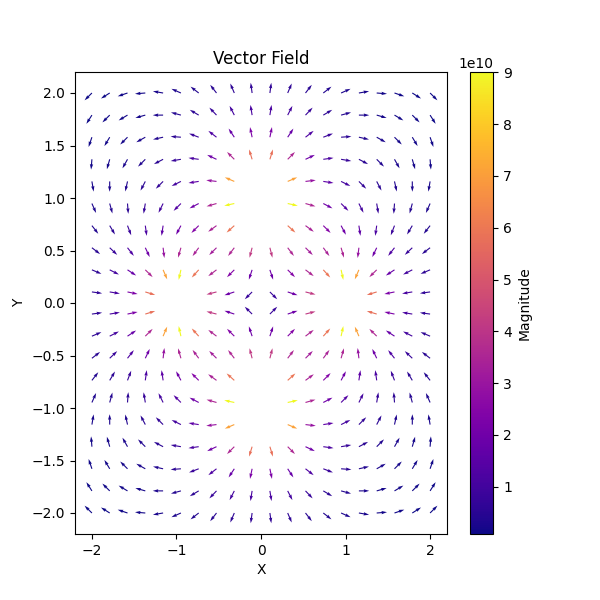
\includegraphics[width=0.6\columnwidth]{figs/field.png}
    \caption{Field Lines}
   \label{label}
\end{figure}
\pagebreak
To find the total electric field at a point in space due to these charges, you add the individual fields (by superposition):
\begin{align*}
E_{\text{total}} = E_1 + E_2 + E_3 + E_4
\end{align*}
\textbf{(b)} Electric Potential may be derived from Electric field by the relation $E = -\nabla V$

1. Electric Potential due to the charge $ +1\,\mathrm{C} $ at $ (0, 1) $:
   \begin{align*}
   V_1 = \frac{1}{4\pi\epsilon_0} \frac{1}{\sqrt{x^2 + (y-1)^2}}
   \end{align*}

2. Electric Potential due to the charge $ +1\,\mathrm{C} $ at $ (0, -1) $:
   \begin{align*}
   V_2 = \frac{1}{4\pi\epsilon_0} \frac{1}{\sqrt{x^2 + (y+1)^2}}
   \end{align*}

3. Electric Potential due to the charge $ -1\,\mathrm{C} $ at $ (1, 0) $:
   \begin{align*}
   V_3 = -\frac{1}{4\pi\epsilon_0} \frac{1}{\sqrt{(x-1)^2 + y^2}}
   \end{align*}

4. Electric Potential due to the charge $ -1\,\mathrm{C} $ at $ (-1, 0) $:
   \begin{align*}
   V_4 = -\frac{1}{4\pi\epsilon_0} \frac{1}{\sqrt{(x+1)^2 + y^2}}
   \end{align*}
\begin{figure}[h!]
   \centering
   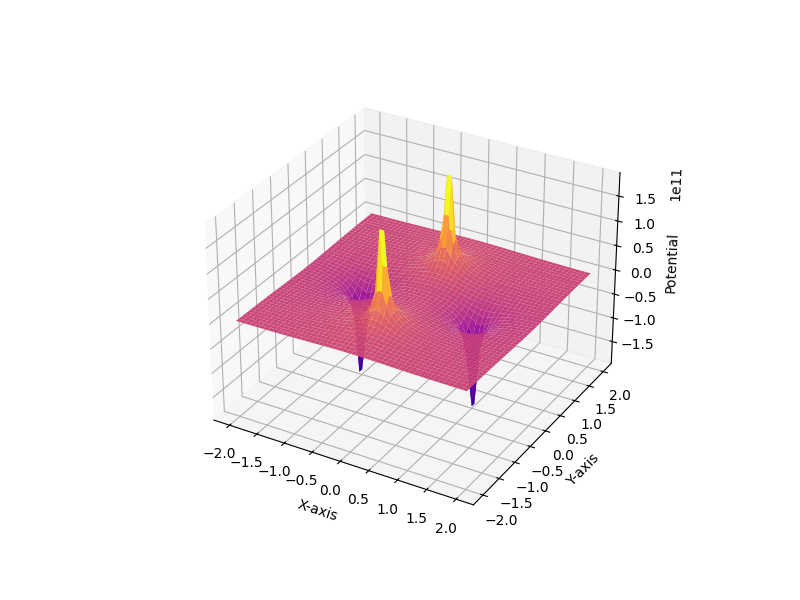
\includegraphics[width=0.6\columnwidth]{figs/pot.png}
    \caption{{Potential Plot}}
   \label{label}
\end{figure}
\pagebreak
To find the total electric potential at a point in space due to these charges, you add the individual potentials (by superposition):
\begin{align*}
V_{\text{total}} = V_1 + V_2 + V_3 + V_4
\end{align*}
   \textbf{(c)}The potential energy of a system of point charges is given by:
\begin{align*}
U = \frac{1}{4\pi\epsilon_0} \sum_{i < j} \frac{q_i q_j}{r_{ij}}.
\end{align*}
In the give question there are 4 charges,
\begin{itemize}
    \item $1C$ at $(0,1)$ and $(0,-1)$.
    \item $-1C$ at $(1,0)$ and $(-1,0)$.
\end{itemize}

Summing up their contributions toward Potential Energy of system,
\begin{align*}
    U &= \frac{1}{4\pi\epsilon_0} \left[ \frac{(1C)(-1C)}{\sqrt{2}} + \frac{(1C)(-1C)}{\sqrt{2}} + \frac{(1C)(-1C)}{\sqrt{2}} + \right. \\ 
    &\left. \frac{(1C)(-1C)}{\sqrt{2}} + \frac{(1C)(1C)}{2} + \frac{(-1C)(-1C)}{2} \right].
\end{align*}

Simplifying:
\begin{align*}
    U &= \frac{1}{4\pi\epsilon_0} \left[ -\frac{4}{\sqrt{2}} + \frac{1}{2} + \frac{1}{2} \right] \\
    &= \frac{q^2}{4\pi\epsilon_0} \left[ 1 - 2\sqrt{2} \right].
\end{align*}

Thus, the potential energy of the configuration is:
\begin{align*}
U = \frac{q^2}{4\pi\epsilon_0} (1 - 2\sqrt{2}).
\end{align*}

\textbf{(d)} Divergence of the electric field\\
The electric field $\mathbf{E}$ due to a point charge $q$ at position $\mathbf{r}_0$ is given by:
\begin{align*}
    \mathbf{E} = \frac{1}{4\pi\varepsilon_0} \frac{q (\mathbf{r} - \mathbf{r}_0)}{|\mathbf{r} - \mathbf{r}_0|^3}.
\end{align*}

By the superposition principle, the total electric field $\mathbf{E}$ is the sum of the contributions from all four charges.

The divergence of the electric field is given by Gauss's law:
\begin{align*}
    \nabla \cdot \mathbf{E} = \frac{\rho}{\varepsilon_0},
\end{align*}
where $\rho(\mathbf{r})$ is the charge density.

Since we have point charges, we can use the Dirac delta function to represent charge density:
\begin{align*}
    \rho(\mathbf{r}) = q \delta(x)\delta(y - 1) + q \delta(x)\delta(y + 1) - q \delta(x - 1)\delta(y) - q \delta(x + 1)\delta(y).
\end{align*}

Applying Gauss's law,
\begin{align*}
    \nabla \cdot \mathbf{E} = \frac{q}{\varepsilon_0} \left[ \delta(x)\delta(y - 1) + \delta(x)\delta(y + 1) - \delta(x - 1)\delta(y) - \delta(x + 1)\delta(y) \right].
\end{align*}

This expression shows that the divergence of field $\mathbf{E}$ is nonzero only at the locations of the charges. This verifies the fact that field due to point charges satisfy Gauss law (in differential form) 

\textbf{(e)} The curl of a vector field $\mathbf{E} = (E_x, E_y, E_z)$ is given by,
\begin{align*}
\nabla \times \mathbf{F} = \begin{vmatrix}
\hat{i} & \hat{j} & \hat{k} \\
\frac{\partial}{\partial x} & \frac{\partial}{\partial y} & \frac{\partial}{\partial z} \\
E_x & E_y & E_z
\end{vmatrix}
\end{align*}

For a single point charge, the electric field components in Cartesian coordinates are:
\begin{align*}
    E_x = \frac{q}{4\pi\varepsilon_0} \frac{x - x_0}{r^3},
\end{align*}

\begin{align*}
    E_y = \frac{q}{4\pi\varepsilon_0} \frac{y - y_0}{r^3},
\end{align*}
\begin{align*}
    E_z = \frac{q}{4\pi\varepsilon_0} \frac{z - z_0}{r^3}.
\end{align*}
where, 
\begin{align*}
    r = [(x - x_0)^2 + (y - y_0)^2 + (z - z_0)^2]^{1/2}
\end{align*}
The curl becomes,
\begin{align*}
    \left( \frac{q}{4\pi\varepsilon_0} \left[ \frac{-3(z - z_0)(y - y_0)}{(r^2)^{5/2}} \right] - \frac{q}{4\pi\varepsilon_0} \left[ \frac{-3(y - y_0)(z - z_0)}{(r^2)^{5/2}} \right] \right)\hat{i } - \\
    \left( \frac{q}{4\pi\varepsilon_0} \left[ \frac{-3(z - z_0)(x - x_0)}{(r^2)^{5/2}} \right] -  \frac{q}{4\pi\varepsilon_0} \left[ \frac{-3(x - x_0)(z - z_0)}{(r^2)^{5/2}} \right]  \right)\hat{j} + \\
    \left( \frac{q}{4\pi\varepsilon_0} \left[ \frac{-3(y - y_0)(x - x_0)}{(r^2)^{5/2}} \right] - \frac{q}{4\pi\varepsilon_0} \left[ \frac{-3(x - x_0)(y - y_0)}{(r^2)^{5/2}} \right]  \right)
\end{align*}
Thus, we get,
\begin{align*}
    \nabla \times \mathbf{E} = \mathbf{0}.
\end{align*}
Since the curl of the field due to a single point charge is zero, and curl operator is linear, the total electric field (which is a superposition of fields of the induvidual charges) also has zero curl.
\begin{align*}
    \nabla \times \mathbf{E} = 0.
\end{align*}

This shows that the electric field due to the system of charges is conservative, i.e. its curl is $0$ \newline \newline
7. Given the spherically symmetric potential field in free space, 
\begin{align*}
V(r) &= V_0 e^{-r/a},
\end{align*}
determine the following:

\begin{enumerate}
    \item[(a)] Find the charge density $\rho_v$ at $r = a$.
    \item[(b)] Calculate the electric field $\mathbf{E}$ at $r = a$.
    \item[(c)] Compute the total charge.
\end{enumerate}
\textbf{Solution:}\newline
\textbf{(a)} Poisson's Equation is given by,
\begin{align*}
\nabla^2 V(r) &= -\frac{\rho(r)}{\epsilon_0}
\end{align*}
In spherical coordiantes,
\begin{align*}
\nabla^2 \phi(r, \theta, \phi) = \frac{1}{r^2} \frac{\partial}{\partial r} \left( r^2 \frac{\partial \phi}{\partial r} \right) + \frac{1}{r^2 \sin \theta} \frac{\partial}{\partial \theta} \left( \sin \theta \frac{\partial \phi}{\partial \theta} \right) + \frac{1}{r^2 \sin^2 \theta} \frac{\partial^2 \phi}{\partial \phi^2} = -\frac{\rho}{\epsilon_0}
\end{align*}

Simplifying:
\begin{align*}
\frac{1}{r^2} \frac{\partial}{\partial r} \left( r^2 \frac{\partial V}{\partial r} \right) 
&= -\frac{\rho(r)}{\epsilon_0}.
\end{align*}

Substituting $V(r) = V_0 e^{-\frac{r}{a}} $:
\begin{align*}
-\frac{V_0 e^{-r/a}}{ar^2} \left( \frac{-r^2}{a} + 2r \right) &= -\frac{\rho(r)}{\epsilon_0}.
\end{align*}

\begin{align*}
\rho(r) &= -\frac{V_0 \epsilon_0 e^{-r/a}}{a}\left( \frac{1}{a} - \frac{2}{r} \right)
\end{align*}
At $ r = a $
\begin{align*}
    \rho = \frac{V_0 \epsilon_0e^{-\frac{r}{a}}}{a^2}
\end{align*}
\textbf{(b)}
\begin{align*}
E &= -\nabla \Phi,
\end{align*}
where $ \Phi $: Potential, $ E $: Electric Field. \newline
Gradient in spherical coordinates,
\begin{align*}
\nabla f(r, \theta, \phi) = & \, \hat{e}_r \frac{\partial f}{\partial r}
                            + \hat{e}_\theta \frac{1}{r} \frac{\partial f}{\partial \theta} 
                            + \hat{e}_\phi \frac{1}{r \sin \theta} \frac{\partial f}{\partial \phi}
\end{align*}

Substituting:
\begin{align*}
E(r) &= \frac{V_0 e^{-\frac{r}{a}}}{a} \hat{r}.
\end{align*}

At $ r = a $:
\begin{align*}
E(r=a) &= \frac{V_0 e^{-1}}{a} \hat{r}.
\end{align*}

\textbf{(c)} Total charge is given by:
\begin{align*}
Q &= \iiint \rho \, dV,
\end{align*}
where $\rho = \text{charge density}$.

\begin{align*}
\rho &= -V_0 \frac{\epsilon_0 e^{-\frac{r}{a}}}{a} \left( \frac{1}{a} - \frac{2}{r} \right).
\end{align*}

Substitute into the integral:
\begin{align*}
Q &= \iiint -V_0 \frac{\epsilon_0}{a} \left( \frac{1}{a} - \frac{2}{r} \right) dV.
\end{align*}

Using spherical coordinates:
\begin{align*}
Q &= \int_{0}^{\infty} \int_{0}^{\pi} \int_{0}^{2\pi} -V_0 \frac{\epsilon_0}{a} 
\left( \frac{1}{a} - \frac{2}{r} \right) r^2 \sin\theta \, dr \, d\theta \, d\phi.
\end{align*}
Analysing the first integral seperately, and applying integration by-parts on the first part
\begin{align*}
&= -V_0 \frac{\epsilon_0}{a} 
\left[ 
    \frac{1}{a}\int_{0}^{\infty} r^2 e^{-\frac{r}{a}} dr 
    - 
    2\int_{0}^{\infty} r e^{-\frac{r}{a}} dr
\right] \\
&= -V_0 \frac{\epsilon_0}{a} 
\left[ \left( \frac{1}{a}r^2(-a) e^{-\frac{r}{a}}\right)_0^{\infty} +
    \frac{1}{a}\int_{0}^{\infty} 2r(-a) e^{-\frac{r}{a}} dr 
    - 
    2\int_{0}^{\infty} r e^{-\frac{r}{a}} dr
\right] 
&= 0
\end{align*}
Thus, the total charge is zero.\newline \newline
8. A parallel-plate capacitor has plates located at $z = 0$ and $z = d$. The region between the plates is filled with a material that contains a uniform volume charge density $\rho_0$ C/m$^3$ and has permittivity $\epsilon$. Both plates are held at ground potential.
\begin{enumerate}
    \item[(a)] Determine the potential field between the plates.
    \item[(b)] Determine the electric field intensity $\mathbf{E}$ between the plates.
    \item[(c)] Repeat parts (a) and (b) for the case where the plate at $z = d$ is raised to a potential $V_0$, with the plate at $z = 0$ grounded.
\end{enumerate}
\textbf{Solution:}\newline
\begin{figure}[h!]
   \centering
   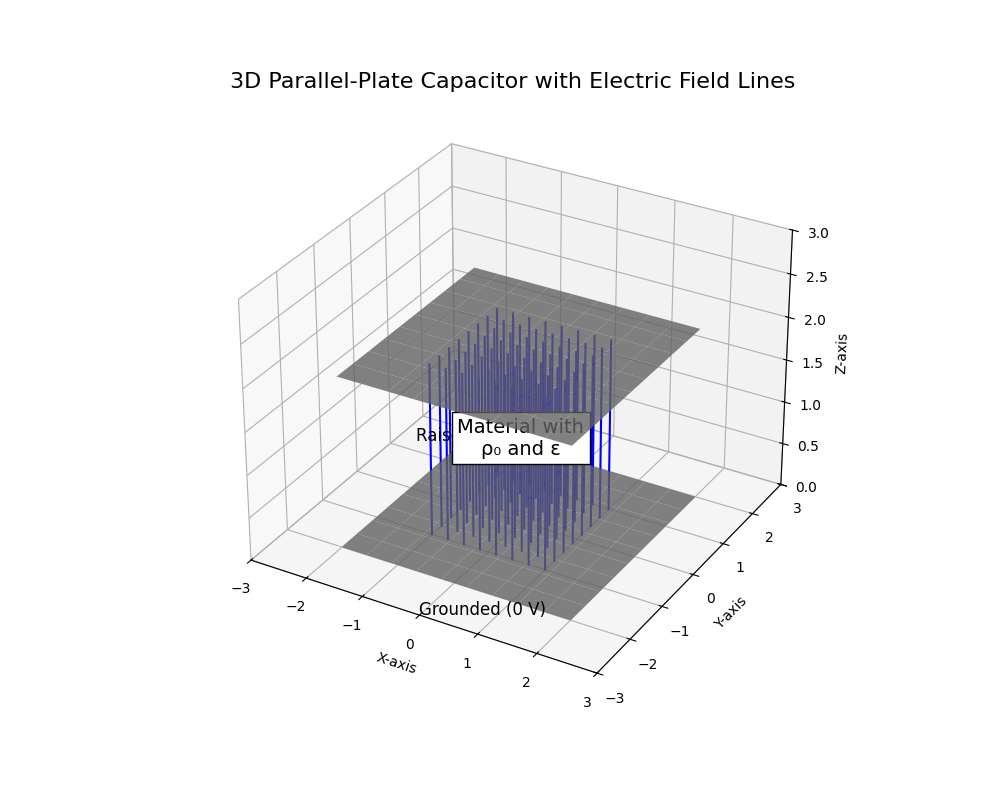
\includegraphics[width=1\columnwidth]{figs/q5.png}
    \caption{capacitor}
   \label{label}
\end{figure}(a) Solving Poisson's Equation
\begin{align*}
    \nabla^2 V &= \frac{\rho}{\epsilon_0} \\
    \text{Here } V \text{ only has a } z \text{ component:} \\
    \frac{d^2 V}{dz^2} &= \frac{\rho}{\epsilon_0} \\
    \frac{dV}{dz} &= \frac{\rho z}{\epsilon_0} + C_1 \\
    V &= \frac{\rho z^2}{2 \epsilon_0} + C_1 z + C_2
\end{align*}

Substituting $ V(z=0) = V(z=d) = 0 $:
\begin{align*}
V = \frac{\rho z (z-d)}{2 \epsilon_0}\hat{k}
\end{align*}

Electric Field Intensity ($E$)
\begin{align*}
E = -\nabla V
\end{align*}
\begin{align*}
E = -\left(-\frac{\rho}{\epsilon_0} \left(z - \frac{d}{2}\right)\right) \quad \hat{k}
\end{align*}

\textbf{(c)}If $V(z=d) = V_0$\newline
From the first part we know,
\begin{align*}
V = \frac{\rho z^2}{2 \epsilon_0} + C_1 z + C_2
\end{align*}
Boundary conditions:
\begin{align*}
V(0) = 0 \implies C_2 = 0
\end{align*}
\begin{align*}
V(d) = V_0 \implies \frac{\rho d^2}{2 \epsilon_0} + C_1 d = V_0
\end{align*}
Solving for $C_1:$
\begin{align*}
C_1 &= \frac{V_0}{d} - \frac{\rho_0 d}{2 \epsilon_0}
\end{align*}
We finally get potential between the plates to be,
\begin{align*}
V &= \left( \frac{\rho_0 z (z-d)}{2 \epsilon_0} + \frac{V_0 z}{d} \right) \hat{r}
\end{align*}
Electric Field Intensity $(\vec{E})$ is given by,
\begin{align*}
\vec{E} &= -\nabla V \\
\vec{E} &= -\left[ \frac{\rho_0}{\epsilon_0} \left( z - \frac{d}{2} \right) + \frac{V_0}{d} \right]
\end{align*}



\end{document}

